%%%%%%%%%%%%%%%%%%%%%%
\nonstopmode
%%
\documentclass[a4paper,12pt]{article}
%%
% Importing the required packages 
\usepackage{verbatim}       % for including codes and also for better usage of comments
\usepackage{graphicx,subfigure,epsfig,float}
\usepackage{xspace}
\usepackage{array,multirow}
\usepackage{amsmath,amssymb,amstext,amsxtra,amsbsy,amsgen}
\usepackage{hyperref}
\usepackage{caption}
%%
% Sizes and margins
\setlength{\textheight}{10.5 in}
\setlength{\textwidth}{7 in}
\setlength{\oddsidemargin}{-0.25 in} 
\setlength{\evensidemargin}{0.00 in}
\setlength{\topmargin}{-1 in}
\topmargin=-1in
%%
\def\baselinestretch{1.5}
%%
% Macros for the ease of writing the report.
% This file contains a collection of useful macros commonly used by the kinematics and robotics community. 

% Use the command "\input{macrosv1.tex}" to use them in a document. All the macros have been defined so that they can be called without using the math mode delimiter ($) and with xspace. 

%This is version#2 of this document created on 12th September, 2018.
%-----------------------------------------------------------------------------------------------------
%-----------------------------------------------------------------------------------------------------

%\usepackage{xspace}
%\usepackage{amsmath,amssymb,amsfonts}

%-----------------------------------------------------------------------------------------------------

% Generic commands

%% Definition of mathmode bold symbols
\newcommand{\bs}[1]{\ensuremath{\boldsymbol{#1}}\xspace}
\newcommand{\mt}[1]{\ensuremath{{#1}}\xspace}

%-----------------------------------------------------------------------------------------------------

% Vector symbols: lowercase English characters

\newcommand{\ba}{\ensuremath{\bs a}\xspace}
\newcommand{\bb}{\ensuremath{\bs b}\xspace}
\newcommand{\bc}{\ensuremath{\bs c}\xspace}
\newcommand{\bd}{\ensuremath{\bs d}\xspace}
\newcommand{\be}{\ensuremath{\bs e}\xspace}
\newcommand{\bsf}{\ensuremath{\bs f}\xspace}
\newcommand{\bg}{\ensuremath{\bs g}\xspace}
\newcommand{\bh}{\ensuremath{\bs h}\xspace}
\newcommand{\bi}{\ensuremath{\bs i}\xspace}
\newcommand{\bj}{\ensuremath{\bs j}\xspace}
\newcommand{\bk}{\ensuremath{\bs k}\xspace}
\newcommand{\bl}{\ensuremath{\bs l}\xspace}
\newcommand{\bm}{\ensuremath{\bs m}\xspace}
\newcommand{\bn}{\ensuremath{\bs n}\xspace}
\newcommand{\bo}{\ensuremath{\bs o}\xspace}
\newcommand{\bp}{\ensuremath{\bs p}\xspace}
\newcommand{\bq}{\ensuremath{\bs q}\xspace}
\newcommand{\br}{\ensuremath{\bs r}\xspace}
\newcommand{\bfs}{\ensuremath{\bs s}\xspace}
\newcommand{\bt}{\ensuremath{\bs t}\xspace}
\newcommand{\bu}{\ensuremath{\bs u}\xspace}
\newcommand{\bv}{\ensuremath{\bs v}\xspace}
\newcommand{\bw}{\ensuremath{\bs w}\xspace}
\newcommand{\bx}{\ensuremath{\bs x}\xspace}
\newcommand{\by}{\ensuremath{\bs y}\xspace}
\newcommand{\bz}{\ensuremath{\bs z}\xspace}

% Matrix symbols: uppercase English characters

\newcommand{\bA}{\ensuremath{\bs A}\xspace}
\newcommand{\bB}{\ensuremath{\bs B}\xspace}
\newcommand{\bC}{\ensuremath{\bs C}\xspace}
\newcommand{\bD}{\ensuremath{\bs D}\xspace}
\newcommand{\bE}{\ensuremath{\bs E}\xspace}
\newcommand{\bF}{\ensuremath{\bs F}\xspace}
\newcommand{\bG}{\ensuremath{\bs G}\xspace}
\newcommand{\bH}{\ensuremath{\bs H}\xspace}
\newcommand{\bI}{\ensuremath{\bs I}\xspace}
\newcommand{\bJ}{\ensuremath{\bs J}\xspace}
\newcommand{\bK}{\ensuremath{\bs K}\xspace}
\newcommand{\bL}{\ensuremath{\bs L}\xspace}
\newcommand{\bM}{\ensuremath{\bs M}\xspace}
\newcommand{\bN}{\ensuremath{\bs N}\xspace}
\newcommand{\bO}{\ensuremath{\bs O}\xspace}
\newcommand{\bP}{\ensuremath{\bs P}\xspace}
\newcommand{\bQ}{\ensuremath{\bs Q}\xspace}
\newcommand{\bR}{\ensuremath{\bs R}\xspace}
\newcommand{\bS}{\ensuremath{\bs S}\xspace}
\newcommand{\bT}{\ensuremath{\bs T}\xspace}
\newcommand{\bU}{\ensuremath{\bs U}\xspace}
\newcommand{\bV}{\ensuremath{\bs V}\xspace}
\newcommand{\bW}{\ensuremath{\bs W}\xspace}
\newcommand{\bX}{\ensuremath{\bs X}\xspace}
\newcommand{\bY}{\ensuremath{\bs Y}\xspace}
\newcommand{\bZ}{\ensuremath{\bs Z}\xspace}

% Greek letters

%% Mathmode lowercase Greek symbols
\newcommand{\alp}{\ensuremath{\alpha}\xspace}
\newcommand{\bet}{\ensuremath{\beta}\xspace}
\newcommand{\gm}{\ensuremath{\gamma}\xspace}
\newcommand{\del}{\ensuremath{\delta}\xspace}
\newcommand{\eps}{\ensuremath{\epsilon}\xspace}
\newcommand{\zet}{\ensuremath{\zeta}\xspace}
\newcommand{\et}{\ensuremath{\eta}\xspace}
\newcommand{\tht}{\ensuremath{\theta}\xspace}
\newcommand{\iot}{\ensuremath{\iota}\xspace}
\newcommand{\kap}{\ensuremath{\kappa}\xspace}
\newcommand{\lam}{\ensuremath{\lambda}\xspace}
\newcommand{\mmu}{\ensuremath{\mu}\xspace}
\newcommand{\mnu}{\ensuremath{\nu}\xspace}
\newcommand{\mxi}{\ensuremath{\xi}\xspace}
\newcommand{\mpi}{\ensuremath{\pi}\xspace}
\newcommand{\mrho}{\ensuremath{\rho}\xspace}
\newcommand{\sig}{\ensuremath{\sigma}\xspace}
\newcommand{\mtau}{\ensuremath{\tau}\xspace}
\newcommand{\ups}{\ensuremath{\upsilon}\xspace}
\newcommand{\ph}{\ensuremath{\phi}\xspace}
\newcommand{\mchi}{\ensuremath{\chi}\xspace}
\newcommand{\mpsi}{\ensuremath{\psi}\xspace}
\newcommand{\om}{\ensuremath{\omega}\xspace}
\newcommand{\vth}{\ensuremath{\vartheta}\xspace}
\newcommand{\vkap}{\ensuremath{\varkappa}\xspace}
\newcommand{\vpi}{\ensuremath{\varpi}\xspace}
\newcommand{\vrho}{\ensuremath{\varrho}\xspace}
\newcommand{\vsig}{\ensuremath{\varsigma}\xspace}
\newcommand{\vph}{\ensuremath{\varphi}\xspace}
\newcommand{\veps}{\ensuremath{\varepsilon}\xspace}

%% Mathmode bold lowercase Greek symbols 
\newcommand{\balp}{\ensuremath{\bs \alpha}\xspace}
\newcommand{\bbet}{\ensuremath{\bs \beta}\xspace}
\newcommand{\bgamma}{\ensuremath{\bs \gamma}\xspace}
\newcommand{\bdel}{\ensuremath{\bs \delta}\xspace}
\newcommand{\beps}{\ensuremath{\bs \epsilon}\xspace}
\newcommand{\bzet}{\ensuremath{\bs \zeta}\xspace}
\newcommand{\bfeta}{\ensuremath{\bs \eta}\xspace}
\newcommand{\bth}{\ensuremath{\bs \theta}\xspace}
\newcommand{\biot}{\ensuremath{\bs \iota}\xspace}
\newcommand{\bkap}{\ensuremath{\bs \kappa}\xspace}
\newcommand{\blam}{\ensuremath{\bs \lambda}\xspace}
\newcommand{\bmu}{\ensuremath{\bs \mu}\xspace}
\newcommand{\bnu}{\ensuremath{\bs \nu}\xspace}
\newcommand{\bxi}{\ensuremath{\bs \xi}\xspace}
\newcommand{\bpi}{\ensuremath{\bs \pi}\xspace}
\newcommand{\brho}{\ensuremath{\bs \rho}\xspace}
\newcommand{\bsig}{\ensuremath{\bs \sigma}\xspace}
\newcommand{\btau}{\ensuremath{\bs \tau}\xspace}
\newcommand{\bups}{\ensuremath{\bs \upsilon}\xspace}
\newcommand{\bphi}{\ensuremath{\bs \phi}\xspace}
\newcommand{\bch}{\ensuremath{\bs \chi}\xspace}
\newcommand{\bpsi}{\ensuremath{\bs \psi}\xspace}
\newcommand{\bom}{\ensuremath{\bs \omega}\xspace}
\newcommand{\bveps}{\ensuremath{\bs \varepsilon}\xspace}
\newcommand{\nvph}{\ensuremath{\bs \varphi}\xspace}
\newcommand{\bvsig}{\ensuremath{\bs \varsigma}\xspace}
\newcommand{\bvrho}{\ensuremath{\bs \varrho}\xspace}
\newcommand{\bvpi}{\ensuremath{\bs \varpi}\xspace}
\newcommand{\bvkap}{\ensuremath{\bs \varkappa}\xspace}
\newcommand{\bvth}{\ensuremath{\bs \vartheta}\xspace}

%% Mathmode uppercase Greek symbols
\newcommand{\Gm}{\ensuremath{\Gamma}\xspace}
\newcommand{\Del}{\ensuremath{\Delta}\xspace}
\newcommand{\Th}{\ensuremath{\Theta}\xspace}
\newcommand{\Lam}{\ensuremath{\Lambda}\xspace}
\newcommand{\mXi}{\ensuremath{\Xi}\xspace}
\newcommand{\mPi}{\ensuremath{\Pi}\xspace}
\newcommand{\Sig}{\ensuremath{\Sigma}\xspace}
\newcommand{\Ups}{\ensuremath{\Upsilon}\xspace}
\newcommand{\Ph}{\ensuremath{\Phi}\xspace}
\newcommand{\Ps}{\ensuremath{\Psi}\xspace}
\newcommand{\Om}{\ensuremath{\Omega}\xspace}

%% Mathmode bold uppercase Greek symbols
\newcommand{\bGm}{\ensuremath{\bs \Gamma}\xspace}
\newcommand{\bDel}{\ensuremath{\bs \Delta}\xspace}
\newcommand{\bTh}{\ensuremath{\bs \Theta}\xspace}
\newcommand{\bLam}{\ensuremath{\bs \Lambda}\xspace}
\newcommand{\bXi}{\ensuremath{\bs \Xi}\xspace}
\newcommand{\bPi}{\ensuremath{\bs \Pi}\xspace}
\newcommand{\bSig}{\ensuremath{\bs \Sigma}\xspace}
\newcommand{\bUps}{\ensuremath{\bs \Upsilon}\xspace}
\newcommand{\bPhi}{\ensuremath{\bs \Phi}\xspace}
\newcommand{\bPsi}{\ensuremath{\bs \Psi}\xspace}
\newcommand{\bOm}{\ensuremath{\bs{\Omega}}\xspace}

% Vector/matrix "zero" and half
\newcommand{\bzero}{\ensuremath{\bs{0}}\xspace}
\newcommand{\half}{\ensuremath{\frac{1}{2}}\xspace}

%-----------------------------------------------------------------------------------------------------

%  Spaces symbols

\newcommand{\C}{\ensuremath{\mathbb{C}}\xspace}
\newcommand{\Cn}{\ensuremath{\mathbb{C}^n}\xspace}
\newcommand{\D}{\ensuremath{\mathbb{D}}\xspace}
\newcommand{\Dn}{\ensuremath{\mathbb{D}^n}\xspace}
\renewcommand{\Re}{\ensuremath{\mathbb{R}}\xspace}
\newcommand{\Rn}{\ensuremath{\mathbb{R}^n}\xspace}
\newcommand{\Ri}[1]{\ensuremath{\mathbb{R}^{#1}}\xspace}
\newcommand{\se}{\ensuremath{se(3)}\xspace}
\newcommand{\ses}{\ensuremath{se^*(3)}\xspace}
\newcommand{\SE}{\ensuremath{\mathbb{SE}(3)}\xspace}
\newcommand{\so}{\ensuremath{so(3)}\xspace}
\newcommand{\SO}{\ensuremath{\mathbb{SO}(3)}\xspace}
\newcommand{\nul}[1]{\ensuremath{\mathcal{N}(#1)}\xspace}
\newcommand{\row}[1]{\ensuremath{\mathcal{R}(#1)}\xspace}


%% Notations for the configuration space
\newcommand{\conf}{\ensuremath{\mathcal{C}}\xspace}
\newcommand{\dimc}{\ensuremath{\textrm{dim}(\mathcal{C})}\xspace}

%-----------------------------------------------------------------------------------------------------

% Jacobian matrices

%% Constraint Jacobian matrices
\newcommand{\jetaq}{\ensuremath{{\boldsymbol J}_{\bfeta\bq}}\xspace}
\newcommand{\jetath}{\ensuremath{{\bs J}_{\bfeta\bth}}\xspace}
\newcommand{\jetaphi}{\ensuremath{{\bs J}_{\bfeta\bphi}}\xspace}
\newcommand{\jetagamma}{\ensuremath{{\bs J}_{\bfeta\bgamma}}\xspace}
\newcommand{\jetapsi}{\ensuremath{{\bs J}_{\bfeta\bpsi}}\xspace}
\newcommand{\jphith}{\ensuremath{{\bs J}_{\bphi\bth}}\xspace}
\newcommand{\jpsith}{\ensuremath{{\bs J}_{\bpsi\bth}}\xspace}
\newcommand{\jgammath}{\ensuremath{{\bs J}_{\bgamma\bth}}\xspace}
\newcommand{\Jfth}{\ensuremath{\boldsymbol{J}_{f\boldsymbol{\theta}}}\xspace}

\newcommand{\jqth}{\ensuremath{{\boldsymbol{J}}_{\bq\bth}}\xspace}
\newcommand{\jpq}{\ensuremath{{\boldsymbol{J}}_{\bp\bq}}\xspace}

\newcommand{\jpcth}{\ensuremath{\boldsymbol{J}_{\pc\bth}\xspace}}
\newcommand{\jpcphi}{\ensuremath{\boldsymbol{J}_{\pc\bphi}\xspace}}
\newcommand{\jpcq}{\ensuremath{\boldsymbol{J}_{\pc\bq}\xspace}}

\newcommand{\jfth}{\ensuremath{\boldsymbol{J}_{\bs{f}\bth}\xspace}}
\newcommand{\jfpsi}{\ensuremath{\boldsymbol{J}_{\bs{f}\bpsi}\xspace}}
\newcommand{\jfrts}{\ensuremath{\boldsymbol{J}_{\bs{f}\bs{r}_{ts}}\xspace}}
\newcommand{\jfpc}{\ensuremath{\boldsymbol{J}_{\bs{f}\bp_c}\xspace}}

\newcommand{\jpth}{\ensuremath{\boldsymbol{J}_{\boldsymbol{p\theta}}\xspace}}
\newcommand{\jpphi}{\ensuremath{\boldsymbol{J}_{\boldsymbol{p\phi}}\xspace}}

%% Angular velocity related
\newcommand{\jom}{\ensuremath{{\bs J}_{\bom}}\xspace}
\newcommand{\jomc}[1]{\ensuremath{{\boldsymbol J}_{\boldsymbol{\omega}_{c_#1}}}\xspace}
\newcommand{\jomth}{\ensuremath{{\bs J}_{\bom\bth}}\xspace}
\newcommand{\jomphi}{\ensuremath{{\bs J}_{\bom\bphi}}\xspace}
\newcommand{\jomeq}{\ensuremath{{\bs J}_{\bom}^{eq}}\xspace}
\newcommand{\jweq}{\ensuremath{{\bs J}_{\bs{w}}^{eq}}\xspace}

%% Linear velocity related
\newcommand{\jv}{\ensuremath{{\bs J}_{\bs v}}\xspace}
\newcommand{\jvp}{\ensuremath{{\bs J}_{{\bs v}{\bs p}}}\xspace}
\newcommand{\jvth}{\ensuremath{{\bs J}_{\bv\bth}}\xspace}
\newcommand{\jvphi}{\ensuremath{{\bs J}_{\bv\bphi}}\xspace}
\newcommand{\jveq}{\ensuremath{{\bs J}_{\bv}^{eq}}\xspace}
\newcommand{\jc}{\ensuremath{{\bs J}_{\bs c}}\xspace}
\newcommand{\jvpc}[1]{\ensuremath{\boldsymbol{J}_{{\bs v}{\bs p}_{c_#1}}}\xspace}
\newcommand{\jcp}{\ensuremath{\bs{J}_{\bs{c}{\bp}}}\xspace}

%-----------------------------------------------------------------------------------------------------

% Kinematics

%% Positions
\newcommand{\rot}[2]{\ensuremath{{}^{#1}_{#2}{\boldsymbol{R}}}\xspace}
\newcommand{\tran}[2]{\ensuremath{{}^{#1}_{#2}{\boldsymbol{T}}}\xspace}
\newcommand{\frm}[1]{\ensuremath{\{#1\}}\xspace}
\newcommand{\pc}{\ensuremath{\boldsymbol{p}_c}\xspace}
\newcommand{\pci}[1]{\ensuremath{\bs{p}_{\boldsymbol{c}_{#1}}}\xspace}

%% Velocities
\newcommand{\vp}{\ensuremath{\bs{v}_{\boldsymbol{p}}}\xspace}
\newcommand{\vpc}[1]{\ensuremath{\bs{v}_{\boldsymbol{p}_{c_#1}}}\xspace}

%% Derivatives
\newcommand{\xd}{\ensuremath{\dot{x}}\xspace}
\newcommand{\xdd}{\ensuremath{\ddot{x}}\xspace}
\newcommand{\bqd}{\ensuremath{\dot{\boldsymbol{q}}}\xspace}
\newcommand{\bqdd}{\ensuremath{\ddot{\boldsymbol{q}}}\xspace}
\newcommand{\pcd}{\ensuremath{\dot{\boldsymbol{p}_c}}\xspace}
\newcommand{\thd}{\ensuremath{\dot{\theta}}\xspace}
\newcommand{\bthd}{\ensuremath{\dot{\bs{\theta}}}\xspace}
\newcommand{\bthdd}{\ensuremath{\ddot{\bth}}\xspace}
\newcommand{\alphad}{\ensuremath{\dot \alpha}\xspace}
\newcommand{\psid}{\ensuremath{\dot{\psi}}\xspace}
\newcommand{\psidd}{\ensuremath{\ddot{\psi}}\xspace}
\newcommand{\phid}{\ensuremath{\dot{\phi}}\xspace}
\newcommand{\bPhid}{\ensuremath{\dot{\bs{\Phi}}}\xspace}
\newcommand{\bphid}{\ensuremath{\dot{\bs{\phi}}}\xspace}
\newcommand{\bpsid}{\ensuremath{\dot{\bs{\psi}}}\xspace}
\newcommand{\bphidr}{\ensuremath{\dot{\boldsymbol{\phi}}^{\textrm{r}}}\xspace}
\newcommand{\bphidn}{\ensuremath{\dot{\boldsymbol{\phi}}^{\textrm{n}}}\xspace}

%-----------------------------------------------------------------------------------------------------.

% Dynamics

\newcommand{\bMth}{\ensuremath{\bs{M_\theta}}\xspace}
\newcommand{\bCth}{\ensuremath{\bs{C_\theta}}\xspace}
\newcommand{\bGth}{\ensuremath{\bs{G_\theta}}\xspace}

\newcommand{\bin}{\ensuremath{\bs{I}_n}\xspace}
\newcommand{\Ith}{\ensuremath{I(\theta)}\xspace}

\newcommand{\bkp}{\ensuremath{\boldsymbol{K}_p}\xspace}
\newcommand{\bkv}{\ensuremath{\boldsymbol{K}_v}\xspace}

\newcommand{\bQc}{\ensuremath{\boldsymbol{Q}^{\textrm{c}}\xspace}}
\newcommand{\Pnc}{\ensuremath{P^{\textrm{nc}}}\xspace}
\newcommand{\bQnca}{\ensuremath{\boldsymbol{Q}^{\textrm{nc}}_{\textrm{a}}\xspace}}
\newcommand{\bQnc}{\ensuremath{\boldsymbol{Q}^{\textrm{nc}}}\xspace}
\newcommand{\bQncr}{\ensuremath{\boldsymbol{\mathcal{Q}}}\xspace}

%-----------------------------------------------------------------------------------------------------.

% Manipulators

\newcommand{\rrs}{\ensuremath{3}-\underline{R}RS\xspace}
\newcommand{\rps}{\ensuremath{3}-R\underline{P}S\xspace}
\newcommand{\upu}{\ensuremath{3}-U\underline{P}U\xspace}
\newcommand{\rrr}{\ensuremath{3}-\underline{R}RR\xspace}
\newcommand{\rpr}{\ensuremath{3}-R\underline{P}R\xspace}
\newcommand{\upsl}{\ensuremath{6}-U\underline{P}S\xspace}
\newcommand{\map}{\mbox{MaPaMan}\xspace}
\newcommand{\mapI}{\mbox{MaPaMan-I}\xspace}
\newcommand{\mapII}{\mbox{MaPaMan-II}\xspace}

%-----------------------------------------------------------------------------------------------------

% Math Symbols

\renewcommand{\iff}{\ensuremath{\mathit{iff}}\xspace}
%\newcommand{\thm}{Theorem}[section]
\newcommand{\imply}{\ensuremath{\Rightarrow \;}\xspace}
\newcommand{\QED}{\ensuremath{\rule[0pt]{1.5ex}{1.5ex}}\xspace}
%\newcommand{\proof}{\noindent\hspace{2em}{\em Proof: }\xspace}
%\newcommand{\endproof}{\hspace*{\fill}~\QED\par\endtrivlist\unskip}
%\newcommand{\mathe}{\verb|Mathematica| \xspace}
\newcommand{\define}{\ensuremath{\stackrel{\Delta}{=}}\xspace}
\newcommand{\elim}[1]{\ensuremath{\stackrel{\times #1}{\longrightarrow}}\xspace}

%% Operations
\newcommand{\adj}{\text{adj}\xspace}
\newcommand{\trace}{\text{tr}\xspace}

%%% Norm
\newcommand{\norm}[1]{\ensuremath{\| #1\|}\xspace}
\newcommand{\normd}[1]{\ensuremath{\| #1\|_d}\xspace}

%%% Partial derivative
\newcommand{\pd}[2]{\ensuremath{\frac{\partial #1}{\partial #2}}\xspace}
\newcommand{\dpd}[2]{\ensuremath{\dfrac{\partial #1}{\partial #2}}\xspace}

%%% Total derivative
\newcommand{\td}[2]{\ensuremath{\frac{\textrm{d} #1}{\textrm{d} #2\hfill}}\xspace}
\newcommand{\dtotder}[2]{\ensuremath{\dfrac{\textrm{d} #1}{\textrm{d} #2\hfill}}\xspace}

%%% Partial second derivative
\newcommand{\pdd}[2]{\ensuremath{\frac{\partial^2 #1}{\partial #2^2}}\xspace}

%%% Total second derivative
\newcommand{\tdd}[2]{\ensuremath{\frac{\textrm{d}^2 #1}{\textrm{d} #2^2\hfill}}\xspace}
\newcommand{\dsecder}[2]{\ensuremath{\dfrac{\textrm{d}^2 #1}{\textrm{d} #2^2\hfill}}\xspace}

%%% Scalar tripple product
\newcommand{\trip}[3]{\ensuremath{\left[#1, #2, #3\right]\xspace}}

%% Rank symbol
\newcommand{\rank}[1]{\ensuremath{\mathrm{rank}\left(#1\right)}\xspace}

%-----------------------------------------------------------------------------------------------------

% Generic words

\newcommand{\dof}{degree-of-freedom\xspace}
\newcommand{\dofs}{degrees-of-freedom\xspace}
\newcommand{\rb}{rigid-body\xspace}
\newcommand{\rbm}{rigid-body motion\xspace}
\newcommand{\asf}{actuator-space formulation\xspace}
\newcommand{\csf}{configuration-space formulation\xspace}

%-----------------------------------------------------------------------------------------------------

\newcommand{\ith}{\ensuremath{i}th\xspace}

%-----------------------------------------------------------------------------------------------------

% References

\newcommand{\mref}[1]{\ref{#1}\xspace}
\newcommand{\mcite}[1]{\cite{#1}\xspace}
\newcommand{\mlabel}[1]{\label{#1}\xspace}

% Quaternions

%%
%New commands
\newcommand{\Hp}{\ensuremath{\stackrel{+}{H}}\xspace}
\newcommand{\Hn}{\ensuremath{\stackrel{-}{H}}\xspace}
% Path for graphics
\graphicspath{{assets/}}
%%
\date{}
\title{Dual Quaternion Based Control}
%\\ED6006: Advanced Topics in the Mechanics of Robots
\author{Akhil Sathuluri}
%ED14B037
%%%%%%%%%%%%%%%%%%%%%
%%
\begin{document}
%
\maketitle % Do not remove this!
%%
\section{Introduction}

\subsection{Why use quaternions?}
The rotation matrices have inherent problems. The following are a few issues using the conventional methods of representation of a rigid body:
\begin{enumerate}
	\item Well known reason of representation singularities using Euler Angles (Gimbal Lock).
	\item The rotational part of the transformation matrix is orthogonal, but they drift and cause unwanted scaling and shearing the object of interest in a computer graphics scenario\cite{ken2012beginners}. Re-normalisation of these matrices is not a simple task. 
	\item Quaternions are useful for another reason that they preserve the algebraic nature of the equations derived from them. They do not produce a complicated set of equations in sines and cosines.
	\item Interpolation of matrices is not straightforward.
\end{enumerate}

\subsubsection{Quaternions}
A short description of quaternions is given below.\\
Quaternion, introduced by Hamilton are four-dimensional extensions to the complex numbers we know. It is represented as,
\begin{align}
	\bq = a_0 + a_1 i+ a_2 j+a_3 k \label{eq1}
\end{align}
where $a_0, a_1, a_2, a_3 \in \Re$ and i, j, k are the imaginary components and are defined as, 
\begin{align}
	i^2=j^2=k^2=-1 \\
	ij=k, jk=i, ki=j, ji=-k, kj=-i, ik=-j
\end{align}
Another common representation of quaternions is as a scalar and a vector pair as shown,
\begin{align}
	\bq = (s, \vec{v})
\end{align} 
The addition of two quaternions follows the normal element wise operation, where as multiplication is as follows, 
\begin{align}
	\bq_1\bq_2 = (s_1 s_2-\vec{v_1}\vec{v_2}, s_1\vec{v_2}+s_2\vec{v_1}+\vec{v_1}\times\vec{v_2})
\end{align}
The conjugate of a quaternion and the norm are as defined, 
\begin{align}
	\bq^* = (s, -\vec{v}) \\
	\norm{\bq} = \bq\bq^*
\end{align}
Unit quaternions, i.e. $\norm{\bq}=1$ can be used to represent rotations. Given rotation of a rigid body by an angle \bth about an axis $\vec{k}$ it can be represented as, 
\begin{align}
	\bq = (cos(\frac{\bth}{2}), \vec{k}sin(\frac{\bth}{2}))
\end{align}

Other useful properties of quaternions are the Hamiltonian operators. For a given quaternion represented as (\ref{eq1}), the Hamiltonian operators are as given \cite{akyar2008dual},
\begin{align}
	\Hp(\bq) = \begin{pmatrix}
	a_0 & -a_1 & -a_2 & -a_3\\
	a_1 &  a_0 & -a_3 &  a_2\\
	a_2 &  a_3 &  a_0 & -a_1\\
	a_3 & -a_2 &  a_1 &  a_0\\	
	\end{pmatrix}
	\\
	\Hn(\bq) = \begin{pmatrix}
	a_0 & -a_1 & -a_2 & -a_3\\
	a_1 &  a_0 &  a_3 & -a_2\\
	a_2 & -a_3 &  a_0 &  a_1\\
	a_3 &  a_2 & -a_1 &  a_0\\	
	\end{pmatrix}
\end{align}

These operators allow us to manipulate the quaternion multiplication as though they are commutative.
\begin{align}
	\bq_1\bq_2 = \Hp(\bq_1) \bq_2 = \Hn(\bq_2) \bq_1 \label{hamilt}
\end{align}

\subsection{Why use dual numbers?}
The reasons for using dual numbers for representation in robot kinematics are, 
\begin{enumerate}
	\item Allows us to do line transformations.
	\item Gives a compact representation of both translation and rotation components, and their velocities, which are represented by a line in the 3D space.
\end{enumerate}
\subsubsection{Dual Numbers}
Given the distance between two lines in 3D as, d and the angle their directions is $\alpha$, 
\begin{align}
	\hat{\alpha} = \alpha + \eps d
\end{align}
where $\eps^2$ is defined to be 0

\subsection{Why use dual quaternions?}
This is a generalisation of a quaternion into a dual number. They carry the advantages of both using quaternions and dual numbers. \\
Unit dual quaternions can be used to represent general affine transformations. and are denoted as below,
\begin{align}
	\hat{\bq} = \bq+\frac{\eps}{2}\bt \bq
\end{align}
where \bq represents the quaternion corresponding to the rotation, \bt represents the quaternion representing translation i.e., (0, $\vec{t}$), where $\vec{t}$ represents the translation vector and $\hat{\bq}$ represents the configuration of a rigid body translated by \bt and then rotated by \bq.

\section{Dual Quaternion Control}
The following method of formulating control law using dual quaternions is as given in \cite{pham2010position}
\subsection{Forward Kinematics}
The robot used in the current study is the six-axis, PUMA 560 robot. The forward kinematic map in terms of the end-effector dual quaternion is obtained based on the DH parameters given in \cite{ghosal2006robotics}
\begin{align}
	\hat{\bq}_{ee} = \hat{\bq}_1\hat{\bq}_2\hat{\bq}_3...\hat{\bq}_n
\end{align}
where, $\hat{\bq}_1$ represents the configuration of the end-effector and the other represent the individual quaternions corresponding to the DH parameters. 
\subsection{Formulating Jacobian}
From here we assume the dual quaternions are mapped to the $\Re^8$. So we differentiate the eight dimensional tuple with respect to the actuated variables, i.e. $\bth_1$, $\bth_2$, $\bth_3$, $\bth_4$, $\bth_5$, $\bth_6$. This gives us a Jacobian of size $8\times6$ which we shall call $J_{dual}$. This gives us,
\begin{align}
	\dot{\hat{\bq}} = J_{dual} \dot{\vec{\bth}} \label{eqJ}
\end{align}
\subsection{Control Law} \label{controllaw}
Here we only deal with a regulation problem using Jacobian based control. A regulation problem is nothing but a position control problem, i.e. given a position or a final configuration, we control the robot to reach that final position. In this case, this is done based on the Jacobian, i.e. the problem is simplified by considering only the kinematics, ignoring the dynamic effects of the robot.
\subsubsection{Error Dynamics}
Let the initial configuration of the end-effector be $\hat{\bq}_1$ and the desired configuration to be $\hat{\bq}_d$. Let us define the error to be,
\begin{align}
	\hat{\bq}_e = \hat{\bq}_d - \hat{\bq} \label{eqe}
\end{align}
where $\hat{\bq}_e$ represents the error dual quaternion and $\hat{\bq}$ represents the configuration at any given instant.\\
Differentiating equation (\ref{eqe}), gives the following,
\begin{align}
	\dot{\hat{\bq}}_e = \dot{\hat{\bq}}_d - \dot{\hat{\bq}}
\end{align}
Since, we are dealing with a regulation problem, we have a fixed $\dot{\hat{\bq}}_d$ and hence its derivative is zero.
\begin{align}
	\dot{\hat{\bq}}_e = - \dot{\hat{\bq}} \label{eqde}
\end{align}
Substituting (\ref{eqJ}) equation in (\ref{eqde}) gives,
\begin{align}
	\dot{\hat{\bq}}_e = - J_{dual} \dot{\vec{\bth}}
\end{align}
Let us consider a proportional control of this system and propose the control law to be,
\begin{align}
	\dot{\vec{\bth}} = J_{dual}^T K \hat{\bq}_e \label{thdyn}
\end{align}
This choice is to ensure asymptotic stability of the system making $J_{dual} J_{dual}^T$ a positive definite matrix\cite{pham2010position}.\\ This gives the error dynamics to be,
\begin{align}
	\dot{\hat{\bq}}_e+J_{dual} J_{dual}^T K \hat{\bq}_e \label{errordyn} = 0 
\end{align}
Integrating the equations (\ref{errordyn}) and (\ref{thdyn}) together gives us the motion of the end-effector.\\
\section{Discussion}
The gain parameter K = 185 is tuned to for the performance parameters of settling time of 10 seconds.\\
The asymptotic convergence of the error is as shown,
\begin{figure}[H]
	\centering
	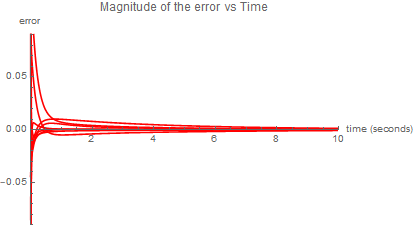
\includegraphics[scale=0.8]{dqc_error}
	\caption{Asymptotic convergence of the quaternion error}
	\label{fg:dqc_error}
\end{figure}
The corresponding plot of the angles reaching the final position is as shown.
\begin{figure}[h]
	\centering
	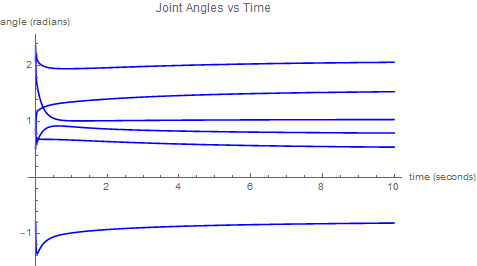
\includegraphics[scale=0.8]{dqc_angles}
	\caption{The trajectory of the six angles of PUMA 560 robot}
	\label{fg:dqc_angles}
\end{figure}
With an increase in the gain as expected the manipulator tries to minimise the error more aggressively.
\section{Utility}
One of the applications for such dual quaternion based control could be in cooperative task space, where two robot arms need to move together to perform a task \cite{adorno2010dual}.\\
When two robots or a single robot with two hands do a task, using dual quaternions to represent the task would greatly simplify the task definition. The paper has suggested the use of various primitives for control. These primitives used in any sequence would give meaningful control to complete the task.\\
One of such primitive is the task definition of relative Cartesian position control which is demonstrated here. Consider the relative quaternion of the end effector to be,
\begin{align}
	\hat{\bq}_r = \hat{\bq}^{*}_{2}\hat{\bq}_{1}\\
	\hat{\bq}_r = \bq_r + \bq^{'}_r\\
	\bq^{'}_r = \frac{\eps}{2}\bt_r \bq_r
\end{align}
Now form this the translation quaternion can be extracted out as, 
\begin{align}
	\bt_r = 2\bq^{'}_r\bq^{*}_r
\end{align}
Again consider the quaternion to be $\bt_r$ to be an element in $\Re^{8}$. Differentiating this equation gives and using (\ref{hamilt}),
\begin{align}
	\dot{\bt_r} = 2\dot{\bq^{'}}_r\bq^{*}_r+2\bq^{'}_r\dot{\bq^{*}_r}\\
	\dot{\bt_r} = 2(\Hn(\bq^{*}_r)J_{\bq^{'}_r}+\Hp(\bq^{'})J_{\bq^{*}_r})\dot{\vec{\bth}}
\end{align}
where $\dot{\vec{\bth}}$ here represents a 12 dimensional vector. So controlling the relative translation quaternion which is 4 dimensional gives us the definition of control for all the joint angles. \\
The similar strategy was used in \cite{adorno2010dual} with four different primitives to perform simple tasks like grasping a balloon and pouring water in a cup from a bottle with a two armed robot.
Using this new definition of Jacobian for the given task, we implement the control strategy as mentioned in section (\ref{controllaw}).
The following is the asymptotic error convergence plot and the corresponding change in the angles of both the manipulators.
\begin{figure}[H]
	\centering
	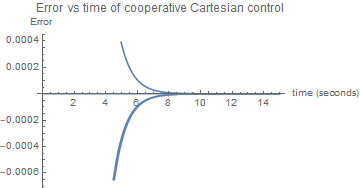
\includegraphics[scale=0.8]{dqc_ctc_error}
	\caption{Asymptotic convergence of the error for relative Cartesian control}
\end{figure}

\section{Error in error}
Based on the (brief) literature survey of usage of dual quaternions done, it is observed that in practical purposes it is comfortable to implement control assuming that these dual quaternions are embedded in $\Re^8$ as in \cite{pham2010position} and \cite{adorno2010dual} to mention a few. But we know that these entities represent elements from \SE, and hence the difference between the two values does not yield a distance measure. It would no longer represent a physically realisable robot configuration as the error is no longer a unit dual quaternion.

\subsection{What do we do?}
For the next part of the work, we follow the path of \cite{bullo1995proportional}, which extends the classical PD controllers to \SO and \SE.\\
Following the formulation in \cite{bullo1995proportional}, we choose to use the logarithmic feedback controller. The setting given in the paper is generic to any system in \SE and an example in $\ensuremath{\mathbb{SE}(2)}\xspace$ of a differential mobile robot is given. In the current work, we extend this formulation to dual quaternions and show its utility in control of a six-axis serial robot.

\section{Error Dynamics}
Knowing the fact that dual quaternions represent elements in \SE, a more reasonable choice of error would be, 
\begin{align}
	\hat{\bq}_e = \hat{{\bq^*}_d} \hat{\bq}
\end{align}
Differentiating the above term and setting $\dot{\hat{\bq}}^*_d$ to zero(regulation problem), we get,
\begin{align}
	\dot{\hat{\bq}}_e = \hat{{\bq^*}_d} \dot{\hat{\bq}}
\end{align}
The logarithmic error feedback in our case would be of the form,
\begin{align}
	\dot{\hat{\bq}} = -K \log(\hat{\bq}_e)
\end{align}
where K is a matrix positive definite matrix. Unlike the previous case, in this case, we can tune the gains for linear and angular velocities separately by internally having different coefficients in the matrix.\\
There are some interesting properties of a dual quaternion. Similar to any complex number which can be represented using the Euler's form, dual quaternions can be represented in a similar way \cite{bottema1979theoretical}.
\begin{align}
	\hat{\bq} = \bq \exp(\eps \frac{\vec{t}}{2})
\end{align}
So applying a logarithm would give us the following, 
\begin{align}
	\log(\hat{\bq}) = \frac{\bth \vec{k}}{2} + \eps \frac{\vec{t}}{2}
\end{align}
Using the above equations, we reformulate the error dynamics in terms of the elements in \se and implement control over these elements.\\
{\bf Note:} Please understand that,
\begin{align}
	\log(\hat{\bq}) = \log(\hat{\bq_1}\hat{\bq_2})
\end{align}
satisfies but, 
\begin{align}
	\log(\hat{\bq}) \neq \log(\hat{\bq_1})+\log(\hat{\bq_2})\\
	\log(\hat{\bq})-\log(\hat{\bq_1}) \neq \log(\hat{\bq_2})
\end{align}
This is from the fact that dual quaternions multiplication is not same as multiplication in $\Re^n$\\
Instead we have, 
\begin{align}
	\log(\hat{\bq^*_1} \hat{\bq}) = \log(\hat{\bq_2})
\end{align}
\section{Discussion}
The error in the controlled entities i.e., the error in end effector orientation and the position asymptotically go to zero.
\begin{figure}[H]
	\centering
	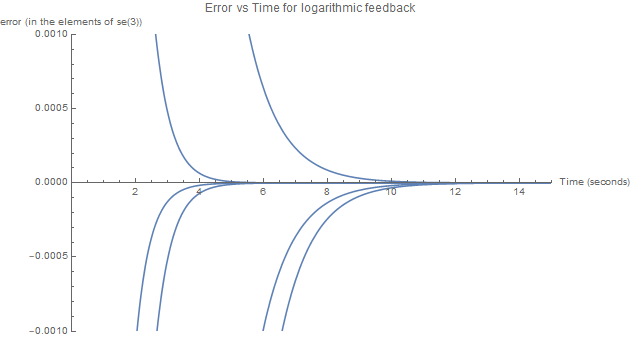
\includegraphics[scale=0.7]{dqc_log_error}
	\caption{Asymptotic convergence of the error for logarithmic feedback}
	\label{fg:dqc_log_error}
\end{figure}
The proportional gain of both the linear and angular velocity components was kept equal to 1 for the above plot.\\
A quick observation is that the variables that converge quickly are the ones corresponding to the errors in the translation of the end-effector. It is also to be noted that the control scheme for position is dependent on the angle at every instant.

\section{Comparison of the two controllers}
Both the controllers were given the same desired, and final quaternion configurations and the resulting control laws are observed. A same gain value is given to both the controllers. We shall call the logarithmic controller as logc and difference controller as diffc from now on.
\begin{figure}[H]
	\centering
	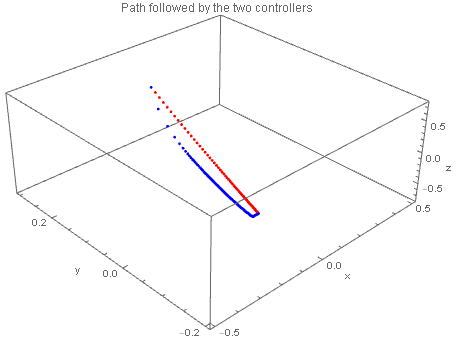
\includegraphics[scale=0.7]{dqc_comparison_path}
	\caption{Path traced by the logarithmic controller (red) and the difference controller(blue)}
	\label{fg:dqc_comparison}
\end{figure}
where the three axes represent $\Re^3$.\\
Note that diffc travels extra distance than the logc. Also that the initial motion of the manipulatior is quite rapid as the dots are farther from each other as compared to the red dots. Investigating the path followed by diffc alone would be as shown below. 
\begin{figure}[H]
	\centering
	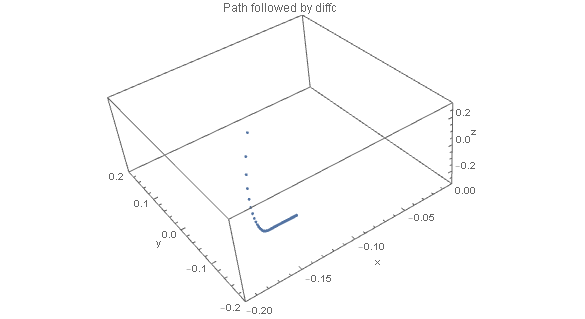
\includegraphics[scale=0.8]{dqc_diffc_path}
	\caption{Curved path traced by diffc}
	\label{fg:dqc_diffc_path}
\end{figure}
The \SE visualisation of the diffc controller is,
\begin{figure}[H]
	\centering
	\begin{subfigure}
		\centering
		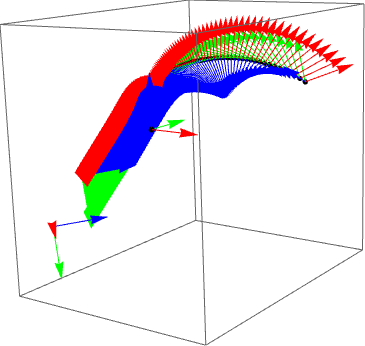
\includegraphics[scale=0.5]{diffc}
		\label{fg:diff_se}
	\end{subfigure}
	\begin{subfigure}
		\centering
		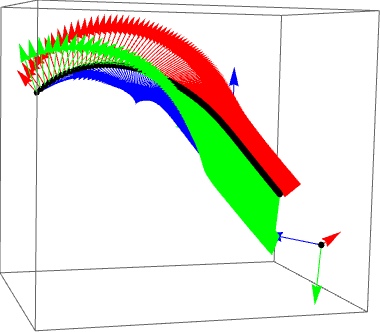
\includegraphics[scale=0.5]{diffc_2}
		\label{fg:diff_se_2}
	\end{subfigure}
	\caption{The \SE visualisation of diffc in two viewing angles}
\end{figure}
The box represents the $\Re^3$. The tri-colour axes represent the \SO part and the black dots represent the $\Re^3$ part of the motion of the manipulator end-effector.

It can be seen that the end-effector does not reach its final configuration in the given time. So increasing the gain to 185 which matches the settling time with logc is as shown, 

\begin{figure}[H]
	\centering
	\begin{subfigure}
		\centering
		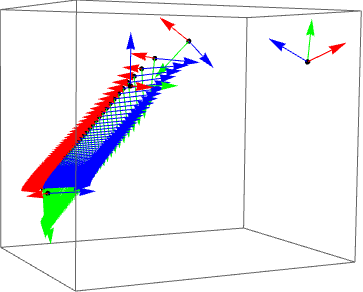
\includegraphics[scale=0.5]{diffc_185}
		\label{fg:logc_se_185}
	\end{subfigure}
	\begin{subfigure}
		\centering
		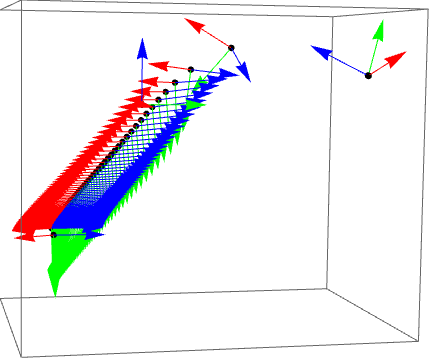
\includegraphics[scale=0.5]{diffc_185_2}
		\label{fg:logc_se_2_185}
	\end{subfigure}
	\caption{The \SE visualisation of logc in two viewing angles for the controller gain of $Kp=185$}
\end{figure}

The initial part of the trajectory is missing in the above plot as the controller was too aggressive in the initial part and the motion took place in a very small time.

The \SE visualisation of the logc controller is,
\begin{figure}[H]
	\centering
	\begin{subfigure}
		\centering
		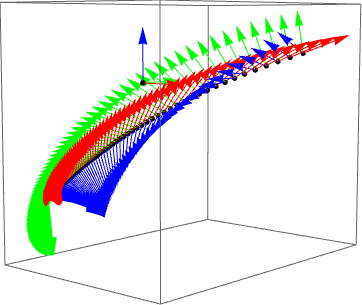
\includegraphics[scale=0.5]{logc}
		\label{fg:logc_se}
	\end{subfigure}
	\begin{subfigure}
		\centering
		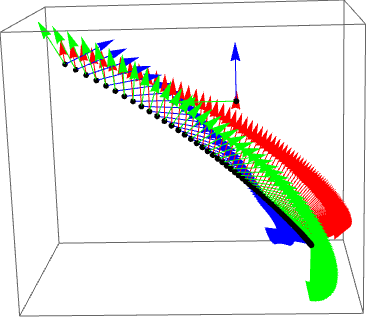
\includegraphics[scale=0.5]{logc_2}
		\label{fg:logc_se_2}
\end{subfigure}
	\caption{The \SE visualisation of logc in two viewing angles}
\end{figure}

So for a given final configuration logc takes a much smaller $Kp$ value 1 compared to the diffc controller which requires a 185, to achieve the same settling time (within 2\% of the final value) of 10s. 

It should also be noted that the logc produces a much less curved solution in $\Re^3$ where as the diffc controller has a comparatively larger curvature. The path of the diffc controller overshoots the final position and comes back to the final configuration, which is a serious trouble in applications like welding and bolting.

The logarithmic controller is arguably in some sense more "natural". 
\section{Concluding question}
Taking this discussion a step further ignoring the internal actuation, dynamics, structure of the hand, I ask the following question,
\begin{center}
	{\bf Our eyes cannot perceive \SE but can our brains do?}\\
	Or does it do even better?
\end{center}
\section{Miscellaneous}
The scope of the current work is as below,
\begin{enumerate}
	\item There is yet another way to describe the error. That is by splitting the \SO and $\Re^3$ parts of the dual quaternion and follow geodesics in each of these space. This approach is called the Double Geodesic Control, which we have not described here.
	\item We have limited ourselves here to a very small subset of the problem. Firstly we deal only with regulation and secondly we are using only a P controller. One could use PD as well, as shown in \cite{bullo1995proportional}.
	\item There is no sense of optimality in the formulation, i.e. we do not extremise any objective here.
	\item Both the controllers behave abruptly as the gain is increased, but the from the error plots and animations, we see that logc closes the gap in Cartesian space and then \SO whereas diffc quickly reaches the orientation and then covers the gap in Cartesian space.
\end{enumerate}
% Bibliography files
\bibliographystyle{ieeetr}
\bibliography{stewart}
%%%
\appendix
\section{Modules}
The following functions are written and used for the completion of the above work.
\subsection{Quaternions}
\begin{enumerate}
	\item quat: Generates a unit quaternion
	\item qmult: Quaternion multiplication
	\item cquat: Conjugate of a given quaternion
	\item Hp: Generates the \Hp of a given quaternion
	\item Hn: Generates the \Hn of a given quaternion
	\item decq: Decomposes a quaternion into axis angle form
\end{enumerate}
\subsection{Dual Quaternions}
\begin{enumerate}
	\item unitdq: Generates a unit dual quaternion
	\item cdualq: Gives the conjugate of a given dual quaternion
	\item dqmult: Dual quaternion multiplication
	\item dHp: Generates \Hp for the corresponding dual quaternion
	\item dHp: Generates \Hn for the corresponding dual quaternion
	\item logdq: Return the logarithm of a dual quaternion
	\item explogdq: Given a logarithm of a dual quaternion it gives the exponent of it
\end{enumerate}
\subsection{Miscellaneous}
\begin{enumerate}
	\item R82dual: Converts an element from $\Re^8$ into a dual quaternion
	\item R62dual: Converts an element from $\Re^6$ into a dual quaternion
	\item frameplotter: Given an element in \se, the module plots the corresponding frame with respect to an origin
\end{enumerate}
\subsection{Initial Conditions}
The non-singular initial and final poses of the manipulator are taken from \cite{ghosal2006robotics}\\

All the modules and the codes can be found in \href{https://github.com/akhilsathuluri/Dual_Quaternion_Control}{my} github page

\end{document}